\section{Historical comparisons with the 2015 and 2016 resonance searches}
\label{app:v501-published-comparisons}

These comparisons use the already analyzed full 2015 and 2016 engineering-run
samples. Here ``95\%'' specifies the confidence level of an upper limit;
``full sample'' specifies the data exposure. Neither term refers to the
unreleased part of the 2021 sample. The curves below are saved historical
results, with their original background models and settings. They provide a
check of the observed yield-to-$\eps^2$ scale and mass-dependent behavior,
while the closure and calibration studies address the separate questions
of bias, signal recovery and coverage.

\subsection{The original and corrected 2015 polynomial analyses}
\label{sec:v501-2015-polynomial-history}

The published 2015 search fitted a Gaussian resonance with the
exponential of a Chebyshev polynomial in a local mass window. Its search covered
approximately \SIrange{19}{81}{MeV}, with fifth-order background below
about \SI{39}{MeV} and third order above. The result used a 95\% confidence
profile-likelihood limit with a power constraint: an observed upper limit
stronger than the median background-only limit was replaced by that
median. Its radiative-fraction convention was $f_{\rm rad}=0.085$
\cite{HPS2015DarkPhoton,HPS2015InternalNote}.

Appendix~J of the 2016 internal note documents a later re-analysis of the
same 2015 sample with the corrected 2016 analysis code
\cite{HPS2016BumpInternal}. The archived account identifies two separate
coordinate-consistency errors in the original implementation. The fit
window was mapped to $[-0.25,0.25]$ instead of the intended $[-1,1]$,
changing the interval over which the polynomial basis had been selected.
The mass resolution was also not consistently transformed from the
physical mass coordinate to the scaled fit coordinate, so the signal
width used by the likelihood was inconsistent with that coordinate.
After those corrections the recorded model choices were
\begin{equation}
 (N,n_\sigma)=
 \begin{cases}
 (5,10),&m_{A^\prime}<\SI{40}{MeV},\\
 (3,8),&m_{A^\prime}\geq\SI{40}{MeV},
 \end{cases}
 \label{eq:v501-corrected-2015-window}
\end{equation}
where $N$ is the polynomial order and $n_\sigma$ is the window-size
parameter reported in the internal note. The corrected contour is its
Fig.~71; its Fig.~72 compares the original and corrected contours.
The corrected re-analysis retained the 2015 detector and radiative inputs
and used the later bounded \CLs{} procedure. It is a distinct reference
from the literal published, power-constrained 2015 curve.

This history is also separate from the RooFit binned extended-likelihood
issue discussed in the 2015 internal note. That note states that its final
results used an independent vanilla ROOT fitter; the coordinate mapping
and signal-width corrections above concern the resonance-search
implementation described in the later internal note
\cite{HPS2015InternalNote,HPS2016BumpInternal}.

\subsection{The historical 2015 GPR comparison}

The original comparison retained in v4.9.7 used a 2015 GPR configuration
with a $2.25\sigma_m$ blind and training-exclusion interval, a
\SI{1}{MeV} mass step, a 7\% radiative-normalization penalty, and the
local event density integrated over the physical
$m\pm1.64\sigma_m$ interval. Its 95\% upper limit used the bounded
profile-likelihood \CLs{} construction. The GP was trained outside
the excluded interval and its count-space background prediction and
correlated uncertainty entered the signal-extraction likelihood. The
Gaussian signal was normalized on the histogram support and sliced into
the extraction window without renormalization, so its amplitude retained
the convention of a total signal yield.

Figure~\ref{fig:v501-2015-method-comparison} restores that earlier
comparison with the corrected 2015 re-analysis. The reference curve was
digitized from the solid black contour in Fig.~71 of the 2016 internal
note. On the common integer-MeV grid from \SIrange{20}{81}{MeV}, the
pointwise ratio
\begin{equation}
 R(m)=\frac{\eps^2_{95,\,\mathrm{GPR}}(m)}
 {\eps^2_{95,\,\mathrm{reference}}(m)}
 \label{eq:v501-historical-limit-ratio}
\end{equation}
has median 0.99 and mean 1.06. The central 68\% of ratios lies
approximately between 0.73 and 1.42, and all but two grid points lie
within a factor of two. This spread is across masses in two observed
curves; it is not a confidence interval or an expected-limit band.

\begin{figure}[p]\centering
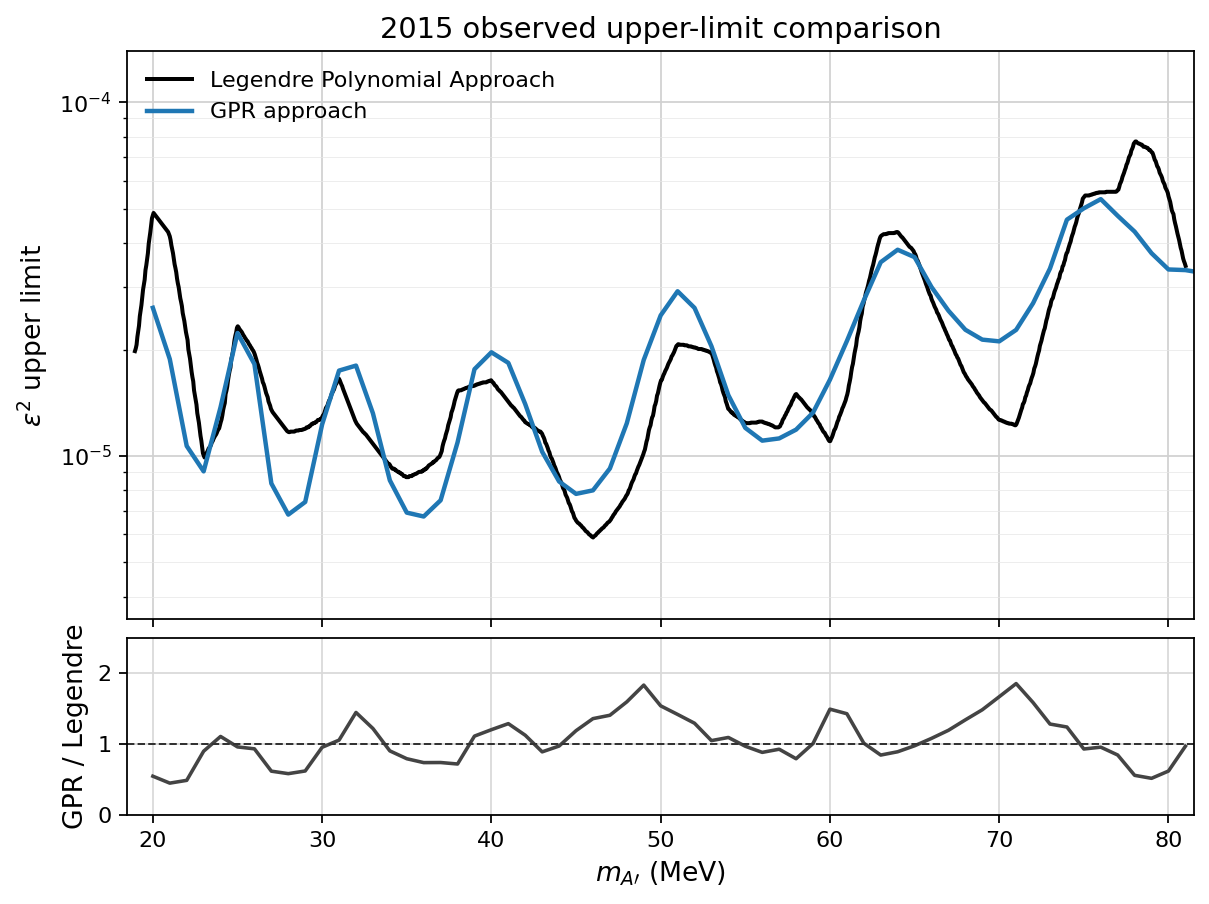
\includegraphics[width=0.98\linewidth]{../figures/history_writer/2015_original_method_comparison.png}
\caption{Restored historical 2015 observed 95\% confidence-limit comparison
from Appendix~E of v4.9.7. The black ``Legendre Polynomial Approach'' curve
is the corrected 2015 re-analysis digitized from Fig.~71 of the 2016
internal note; the blue curve is the earlier GPR comparison for the same
full 2015 sample. The lower panel is the pointwise ratio of these saved
curves, with median 0.99 and mean 1.06 over \SIrange{20}{81}{MeV}.
Both curves predate the current v5 settings. Their similar normalization
scale does not establish coverage or absence of signal absorption.}
\label{fig:v501-2015-method-comparison}
\end{figure}

A separate comparison campaign on 5 August 2026 recomputed the 95\%
limits at the reviewed v4 2015 kernel coordinates with upper
length-scale factor 8. That campaign obtained median ratios of 1.1094
against the literal published 2015 contour and 0.8437 against the
corrected recast. The first comparison used log-linear interpolation
of the published digitization on \SIrange{20}{81}{MeV}; the second
used exact matched masses on \SIrange{19}{81}{MeV}. These later
numbers belong to that later frozen GP state and are not replacements
for the 0.99 ratio in the restored figure.

\subsection{The published 2016 method and the saved GPR comparison}
\label{sec:v501-2016-published-method}

The published 2016 analysis used a Gaussian signal plus an
\emph{exponentiated} Legendre-polynomial background,
\begin{equation}
 f(m)=\mu\,G(m;m_{A^\prime},\sigma_m)
      +10^{L_N(m;\boldsymbol t)},
 \label{eq:v501-2016-polynomial-model}
\end{equation}
with the polynomial evaluated in the coordinate scaled to the local
fit interval. The background is therefore positive; it is not a raw
Legendre polynomial added directly to the signal. The selected order
was five below \SI{66}{MeV} and three above, and the full fit-window
width ranged from six to ten mass resolutions. Windows that reached
the event-range boundaries were shifted to stay within those
boundaries. The published upper limit used the 95\% asymptotic
\CLs{} construction. The reported systematic treatment included
10\,000 variations of the signal width for the 3.4\% resolution
uncertainty, taking the 84th-percentile upper limit, and a downward
7.4\% adjustment of the radiative fraction for its total uncertainty
\cite{HPS2016PromptLong}.

Figure~\ref{fig:v501-2016-95cl-comparison} uses the saved
5 August 2026 GPR comparison. The GPR curve is the historical v4.1
2016 candidate with upper length-scale factor 12, selected through
the boundary-release and likelihood-plateau study described in
Section~\ref{sec:v501-2016-upper-range}. It is not the current
v5 observed curve. For this comparison the reviewed kernel amplitude
and length scale were held fixed, with no optimizer restarts; only
the \CLs{} test size was changed from $\alpha=0.10$ to $0.05$.
The individual 2016 likelihood used fit support
\SIrange{30}{210}{MeV}, search \SIrange{39}{180}{MeV}, and
$2.25\sigma_m$ extraction and training exclusion. The GPR conversion
used its recorded 7\% radiative penalty and the uncropped,
fractional-bin density integral over $m\pm1.64\sigma_m$.
Thus the confidence levels match, while the background treatment and
systematic prescriptions remain different.

\begin{table}[htbp]\centering\small
\begin{tabularx}{\linewidth}{P{0.24\linewidth}YY}
\toprule
Feature & Published 2016 analysis & Archived v4.1 GPR comparison \\
\midrule
Data & Full 2016 engineering-run sample & Same full 2016 sample \\
Background & Local exponentiated Legendre fit; coefficients profiled
with the signal & Sideband-trained log-count GP; predicted count-space
mean and correlated uncertainty enter the extraction \\
Window & Mass-dependent local fit, six to ten resolutions in full width
& GP support 30--210 MeV; local extraction $\pm2.25\sigma_m$ \\
Signal & Gaussian with detector resolution and reported width-systematic
variations & Gaussian normalized on the full histogram support and
sliced into the extraction interval \\
Upper limit & 95\% asymptotic \CLs{} with the published systematic treatment
& 95\% asymptotic bounded-profile \CLs{} at the saved GP coordinates \\
Interpretation & Published observed result & Historical observed diagnostic;
no new toy calibration or expected bands \\
\bottomrule
\end{tabularx}
\caption{Methods entering the saved 2016 comparison. Matching confidence
level and data exposure does not make the two inference procedures identical.}
\label{tab:v501-2016-method-comparison}
\end{table}

The archived reconstruction reproduced the selected 90\% signal-yield
limits with maximum relative difference $1.378\times10^{-10}$ before
the change to 95\%. Updating only the density integral shifted the
corresponding 2016 coupling conversion by $-0.176\%$ to $+0.270\%$;
the likelihood yield was unchanged. No pseudoexperiments or expected
bands were generated for that comparison. On the 141 matched masses
from \SIrange{39}{179}{MeV}, its GPR/published ratio has median
0.5579 and is below one at 117 masses. The minimum and maximum
ratios are 0.2049 at \SI{80}{MeV} and 1.7344 at \SI{160}{MeV}.
The median corresponds to a 44.2\% reduction in the observed limit
on that comparison grid, not a demonstrated 44.2\% sensitivity gain.

Shared counts, resolution and radiative inputs explain part of the
agreement; different background responses and realized fluctuations
can change individual masses. Coverage and signal recovery require
the distinct toy tests in Section~\ref{sec:toys} and
Appendix~\ref{sec:v5-calibration}.

\begin{figure}[p]\centering
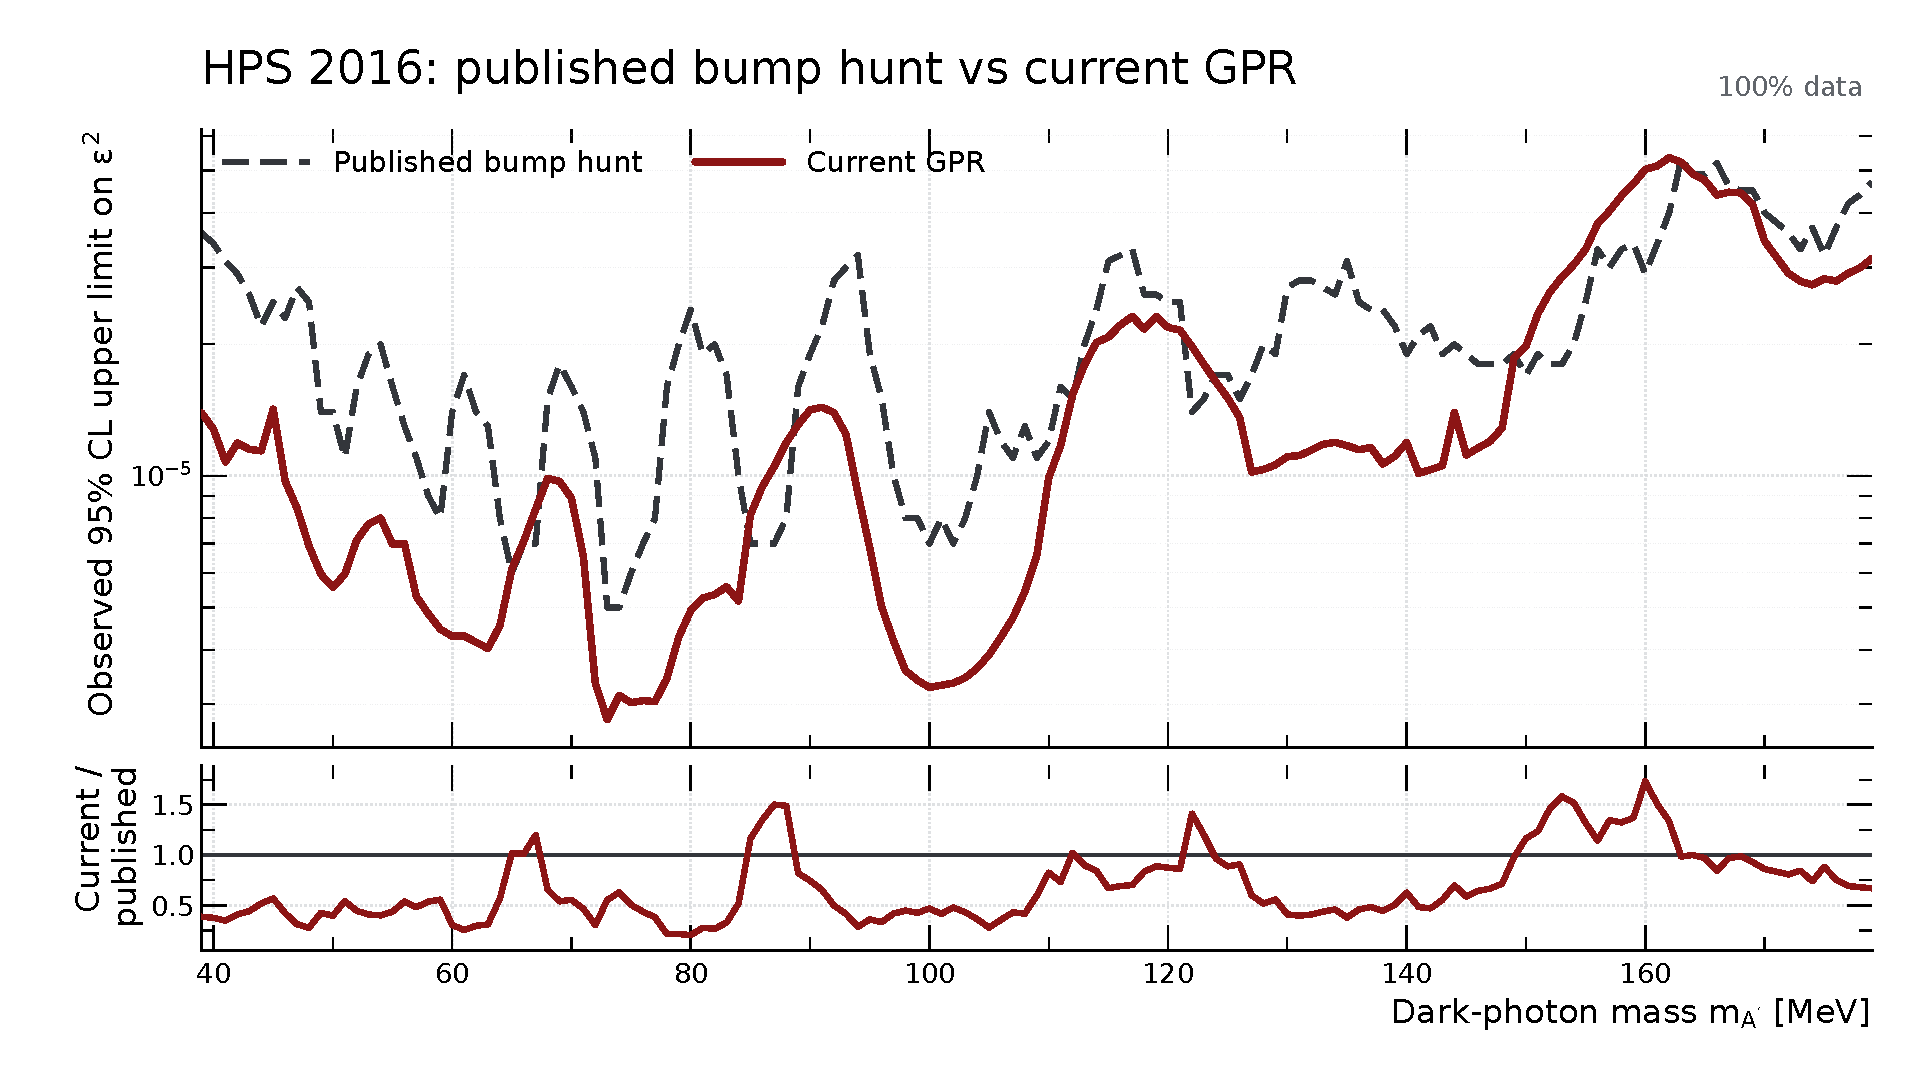
\includegraphics[width=0.99\linewidth]{../figures/history_writer/2016_saved_95cl_comparison.pdf}
\caption{Saved 2016 observed 95\% confidence-limit comparison from
5 August 2026, using the full already analyzed 2016 sample. The
published reference uses the polynomial \CLs{} method; the curve
labeled ``current'' in this archived graphic means the then-current
v4.1 factor-12 GPR candidate. It does not mean the v5.0.1 configuration.
The lower panel gives the pointwise observed GPR/published ratio,
whose median is 0.5579 over 141 matched masses. This was an observed,
asymptotic comparison with fixed reviewed kernel coordinates, no
new toys, and no expected-limit bands.}
\label{fig:v501-2016-95cl-comparison}
\end{figure}
